% !TEX root=../root.tex

\subsection{Feature Tracking}
As mentioned in~\secref{sec:estimation}, in addition to using measurements from the fiducial landing
marker, the estimation algorithm uses measurements of visual features that are
rigidly attached to the landing vehicle. It is important to note that the
problem of determining which visual features in a camera image are attached to
the landing vehicle is not trivial. We leave this problem as future work and
circumvent this problem by flying low enough to the landing vehicle that the
landing vehicle takes up the entire field of view of the camera.

Visual features are first detected using a FAST feature
detector~\cite{rosten2006machine}. Features are then tracked from one frame to
the next using optical flow~\cite{bouguet2001pyramidal}. Periodically, we remove
features that have been tracked poorly by computing the Essential matrix between
the current camera image and a stored keyframe image using RANSAC. Outliers to the found
Essential matrix are thrown out, and new FAST features are detected to replace
them. For our experiements, the feature tracker attempted to maintain 250
tracked features. As the proposed estimator only uses measurements from a few
tracked features, a subset of the features which have been tracked the longest
are provided to the estimator. 

Each visual feature that is acquired and tracked is assigned a unique integer
identitication number. The estimator uses these identification numbers to
determine when a visual feature is no longer tracked and should be removed from
the estimated state.
An example camera image from the UAV showing the
subset of tracked features provided to the estimator and their identificantion
numbers can be seen in~\figref{fig:features_with_aruco}.


\begin{figure}
  \centering
  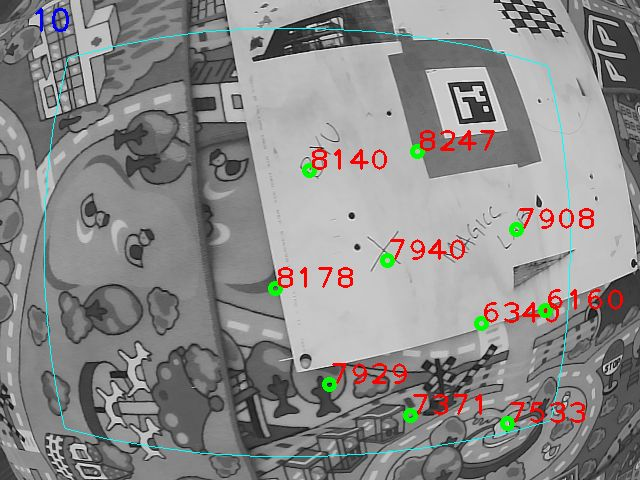
\includegraphics[scale=0.5]{imgs/features_with_aruco.png}
  \caption{A processed camera image from the multirotor UAV's camera. The ArUco
  landing marker is pictured in the top, right corner of the image. Each green
circle shows the tracked location of a visual landmark being used by the
estimator. The red number associated with each visual landmark is the unique
integer ID assigned by the feature tracker.}
  \label{fig:features_with_aruco}
\end{figure}
